Na slici \ref{fig:er} se nalazi detaljan konceptualan model baze podataka.

\begin{figure}[!h]
    \centering
    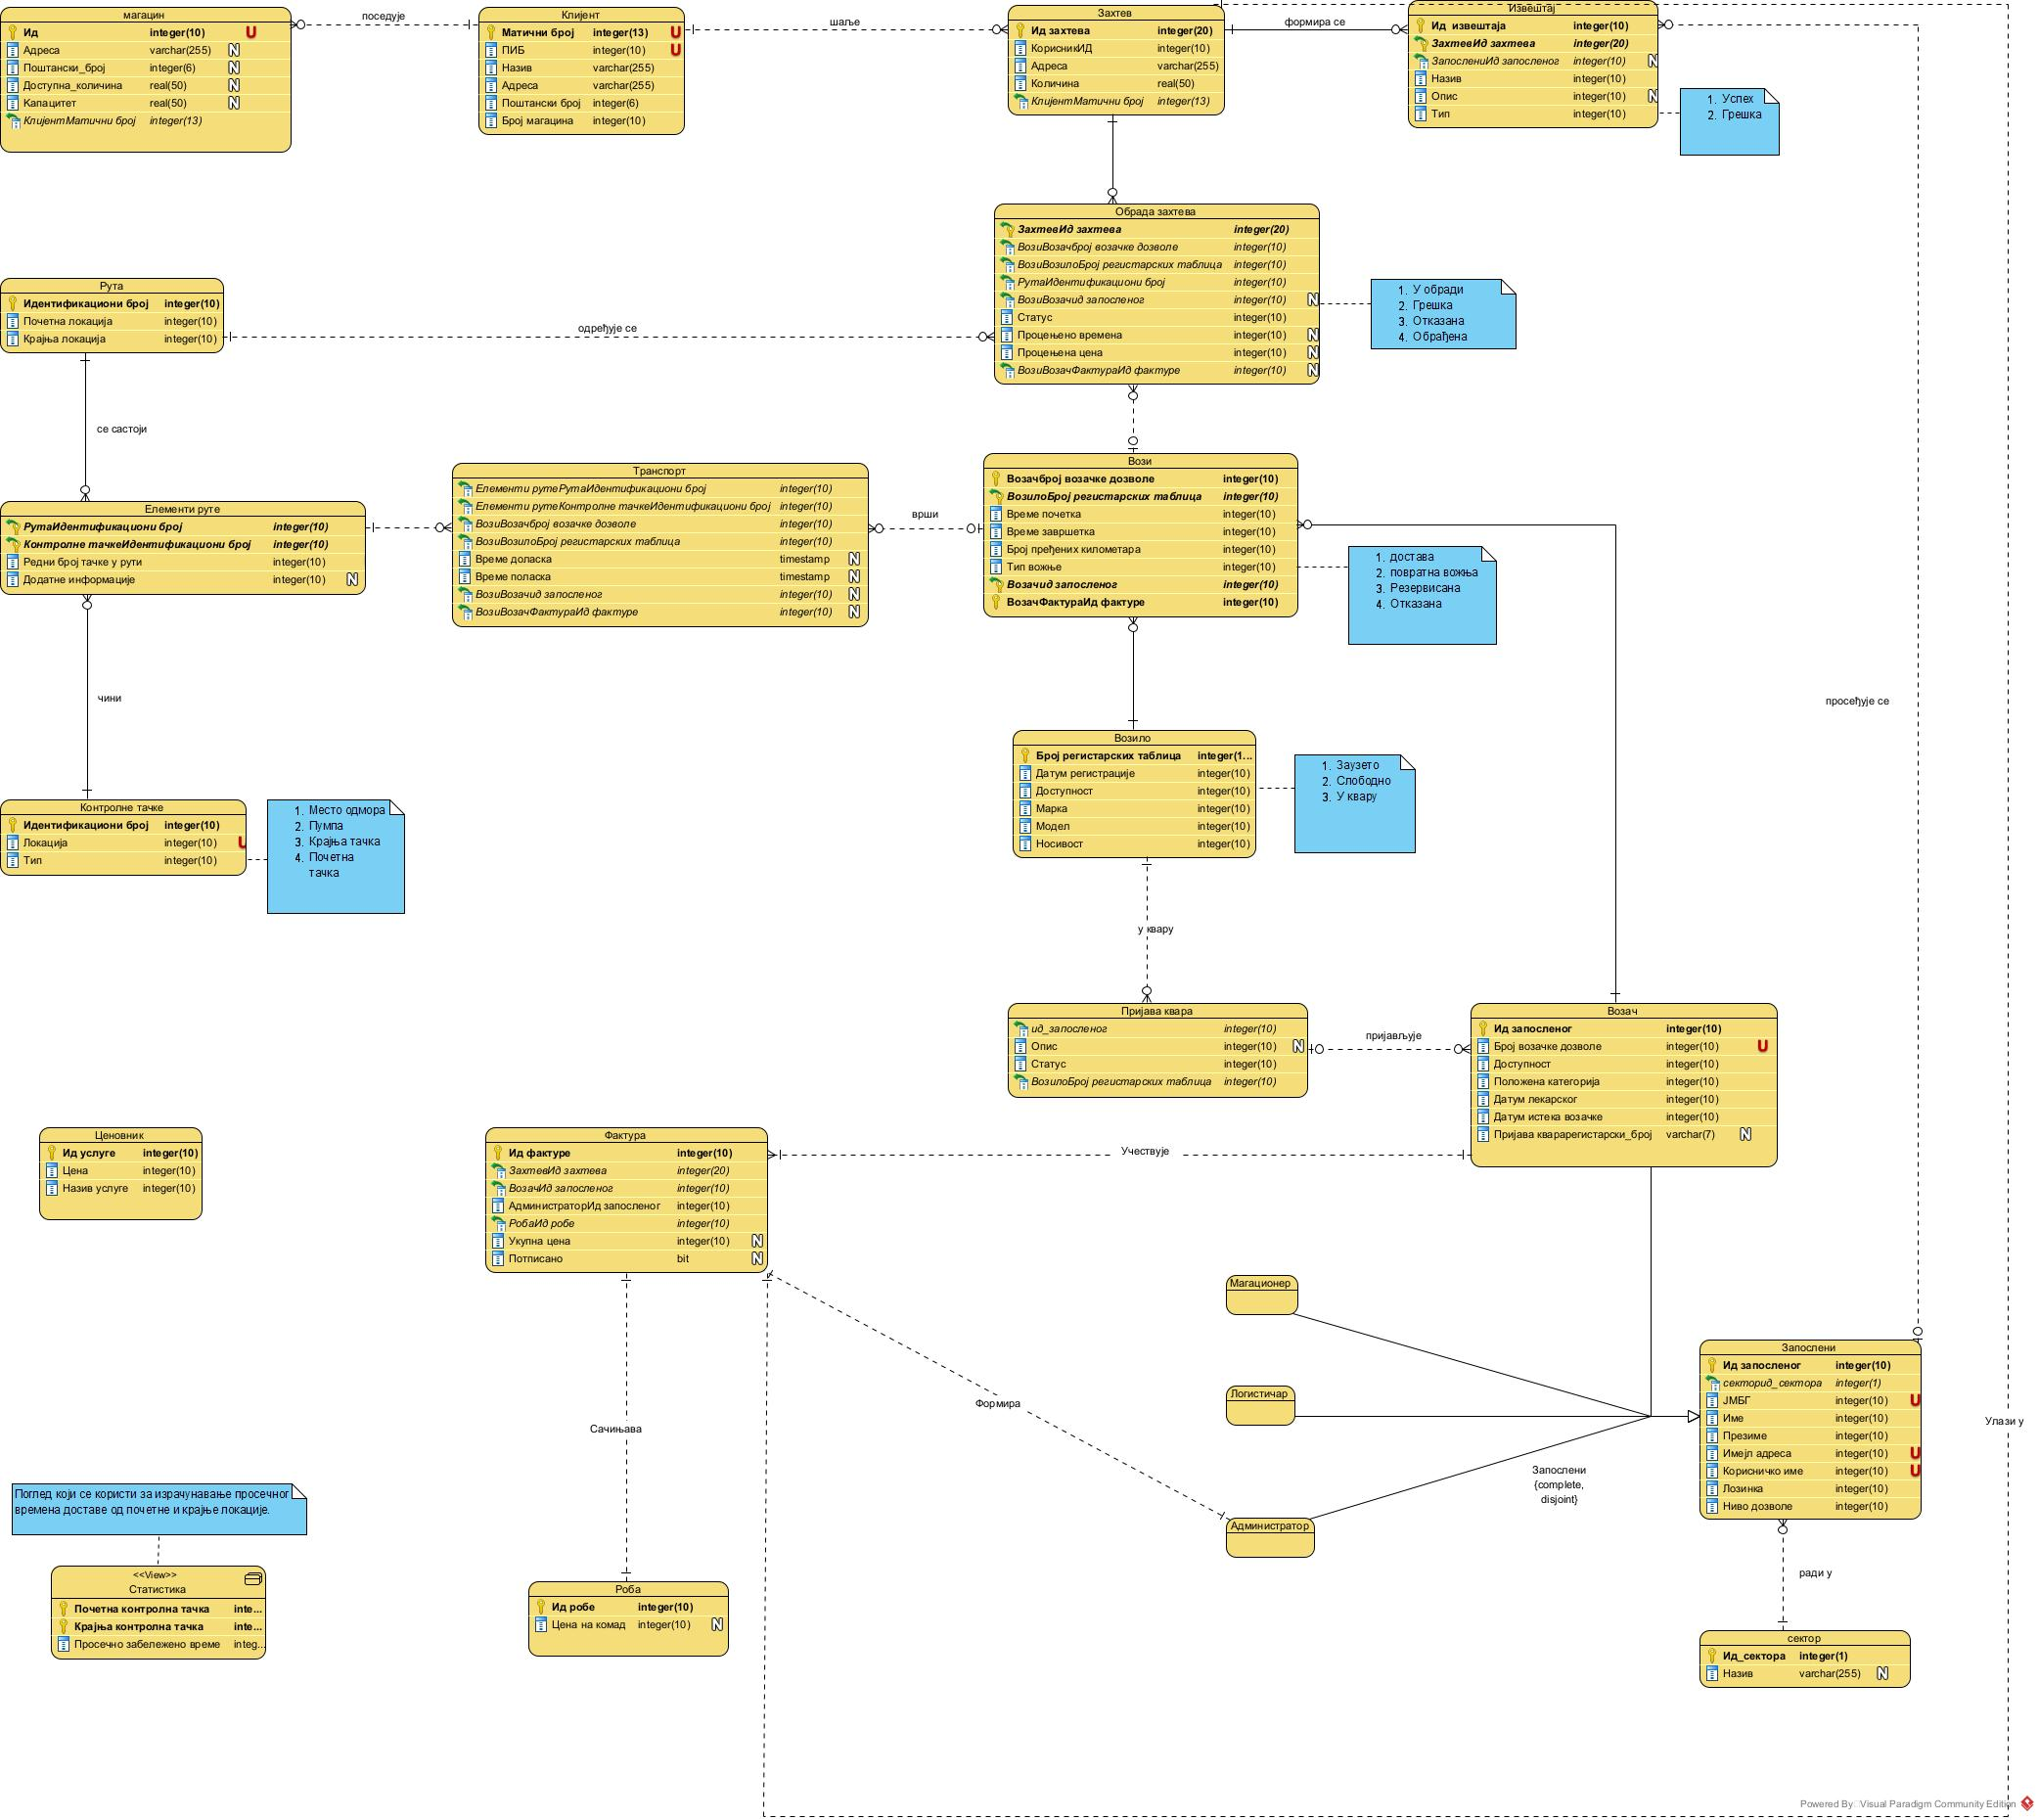
\includegraphics[width=14cm]{Slike/ER.jpg}
    \caption{Dijagram objekti-veze baze podataka}
    \label{fig:er}
\end{figure}

\subsection{Privilegije korisnika}
Sa obzirom na to da sistemu pristupaju razlichiti korisnici, potrebno je prodiskutovati i privilegije koje svaki od njih ima nad bazom podataka prilikom pristupa sistemu i koje je potrebno isposhtovati prilikom fizichke implementacije baze podataka.

\begin{enumerate}
    \item Korisnici, Vozachi i Magacioneri imaju samo privilegije chitanja.
    \item Logistichari mogu da menjaju odredjene informacije vezane za planiranje transporta. Dakle, mogu da dodaju/brishu kljuchne tachke rute, kao i samu rutu, kao i informacije o zahtevu i njegovoj obradi. Ostale informacije mogu samo da chitaju.

    \item Administratori imaju privilegije chitanja, pisanja i menjanja svih informacija.
    
\end{enumerate}
